\documentclass[11pt,reqno,final,pdftex]{amsart}\usepackage[]{graphicx}\usepackage[]{color}
%% maxwidth is the original width if it is less than linewidth
%% otherwise use linewidth (to make sure the graphics do not exceed the margin)
\makeatletter
\def\maxwidth{ %
  \ifdim\Gin@nat@width>\linewidth
    \linewidth
  \else
    \Gin@nat@width
  \fi
}
\makeatother

\definecolor{fgcolor}{rgb}{0.345, 0.345, 0.345}
\newcommand{\hlnum}[1]{\textcolor[rgb]{0.686,0.059,0.569}{#1}}%
\newcommand{\hlstr}[1]{\textcolor[rgb]{0.192,0.494,0.8}{#1}}%
\newcommand{\hlcom}[1]{\textcolor[rgb]{0.678,0.584,0.686}{\textit{#1}}}%
\newcommand{\hlopt}[1]{\textcolor[rgb]{0,0,0}{#1}}%
\newcommand{\hlstd}[1]{\textcolor[rgb]{0.345,0.345,0.345}{#1}}%
\newcommand{\hlkwa}[1]{\textcolor[rgb]{0.161,0.373,0.58}{\textbf{#1}}}%
\newcommand{\hlkwb}[1]{\textcolor[rgb]{0.69,0.353,0.396}{#1}}%
\newcommand{\hlkwc}[1]{\textcolor[rgb]{0.333,0.667,0.333}{#1}}%
\newcommand{\hlkwd}[1]{\textcolor[rgb]{0.737,0.353,0.396}{\textbf{#1}}}%

\usepackage{framed}
\makeatletter
\newenvironment{kframe}{%
 \def\at@end@of@kframe{}%
 \ifinner\ifhmode%
  \def\at@end@of@kframe{\end{minipage}}%
  \begin{minipage}{\columnwidth}%
 \fi\fi%
 \def\FrameCommand##1{\hskip\@totalleftmargin \hskip-\fboxsep
 \colorbox{shadecolor}{##1}\hskip-\fboxsep
     % There is no \\@totalrightmargin, so:
     \hskip-\linewidth \hskip-\@totalleftmargin \hskip\columnwidth}%
 \MakeFramed {\advance\hsize-\width
   \@totalleftmargin\z@ \linewidth\hsize
   \@setminipage}}%
 {\par\unskip\endMakeFramed%
 \at@end@of@kframe}
\makeatother

\definecolor{shadecolor}{rgb}{.97, .97, .97}
\definecolor{messagecolor}{rgb}{0, 0, 0}
\definecolor{warningcolor}{rgb}{1, 0, 1}
\definecolor{errorcolor}{rgb}{1, 0, 0}
\newenvironment{knitrout}{}{} % an empty environment to be redefined in TeX

\usepackage{alltt}
%% DO NOT DELETE OR CHANGE THE FOLLOWING TWO LINES!
%% $Revision$
%% $Date$
\usepackage[round,sort,elide]{natbib}
\usepackage{graphicx}
\usepackage{times}
\usepackage{rotating}
\usepackage{subfig}
\usepackage{color}
\newcommand{\aak}[1]{\textcolor{cyan}{#1}}
\newcommand{\mab}[1]{\textcolor{red}{#1}}
\newcommand{\cec}[1]{\textcolor{blue}{#1}}

\setlength{\textwidth}{6.25in}
\setlength{\textheight}{8.75in}
\setlength{\evensidemargin}{0in}
\setlength{\oddsidemargin}{0in}
\setlength{\topmargin}{-.35in}
\setlength{\parskip}{.1in}
\setlength{\parindent}{0.3in}

%% cleveref must be last loaded package
\usepackage[sort&compress]{cleveref}
\newcommand{\crefrangeconjunction}{--}
\crefname{figure}{Fig.}{Figs.}
\Crefname{figure}{Fig.}{Figs.}
\crefname{table}{Table}{Tables}
\Crefname{table}{Tab.}{Tables}
\crefname{equation}{Eq.}{Eqs.}
\Crefname{equation}{Eq.}{Eqs.}
\crefname{appendix}{Appendix}{Appendices}
\Crefname{appendix}{Appendix}{Appendices}
\creflabelformat{equation}{#2#1#3}

\theoremstyle{plain}
\newtheorem{thm}{Theorem}
\newtheorem{corol}[thm]{Corollary}
\newtheorem{prop}[thm]{Proposition}
\newtheorem{lemma}[thm]{Lemma}
\newtheorem{defn}[thm]{Definition}
\newtheorem{hyp}[thm]{Hypothesis}
\newtheorem{example}[thm]{Example}
\newtheorem{conj}[thm]{Conjecture}
\newtheorem{algorithm}[thm]{Algorithm}
\newtheorem{remark}{Remark}
\renewcommand\thethm{\arabic{thm}}
\renewcommand{\theremark}{}

\numberwithin{equation}{part}
\renewcommand\theequation{\arabic{equation}}
\renewcommand\thesection{\arabic{section}}
\renewcommand\thesubsection{\thesection.\arabic{subsection}}
\renewcommand\thefigure{\arabic{figure}}
\renewcommand\thetable{\arabic{table}}
\renewcommand\thefootnote{\arabic{footnote}}

\newcommand\scinot[2]{$#1 \times 10^{#2}$}
\newcommand{\code}[1]{\texttt{#1}}
\newcommand{\pkg}[1]{\textsf{#1}}
\newcommand{\dlta}[1]{{\Delta}{#1}}
\newcommand{\Prob}[1]{\mathbb{P}\left[#1\right]}
\newcommand{\Expect}[1]{\mathbb{E}\left[#1\right]}
\newcommand{\Var}[1]{\mathrm{Var}\left[#1\right]}
\newcommand{\dd}[1]{\mathrm{d}{#1}}
\newcommand{\citetpos}[1]{\citeauthor{#1}'s \citeyearpar{#1}}
\IfFileExists{upquote.sty}{\usepackage{upquote}}{}
\begin{document}



\section*{Goals}
The task here is to attempt to fit the growth, reproduction, and spore production data from Cat Searle's experiments with \emph{D. dentifera} and \emph{P. ramosa}.
Her experiment used a sacrifice series to quantify spore production at different infection ages, but she also measured size, cumulative reproduction, and, most importantly, clearance rate for the animals sacrificed at each age.
The clearance rate data is especially valuable, as it should allow us to forego needing to fit feeding parameters separately.
(Note to self (see below): clearance rate is calculated assuming a Type I functional response for the \emph{Daphnia}.)
Based on my previous efforts and conversations with other people, the feeding model is both the most difficult to fit, and the values of those parameters will critically affect the best-fit values of other parameters.

The key question is what the model for parasite growth should look like.
My Proc B paper suggested that parasites get energy from the allocation to growth.
Simple carbon accounting in the Proc B paper suggested that the total carbon in spores+tissue was about equal to the amount of carbon liberated by castration (the carbon that should have ended up in eggs).
Moreover, the paper suggested that about 45\% of the liberated carbon ended up in spores.
These observations suggest some potential models for parasite growth, but it would be good to test those explicitly here, using fitting.

The challenge will be figuring out how to model parasite growth/energy theft. A number of possibilities spring to mind:
\begin{itemize}
\item Parasites receive a constant fraction of energy allocated to growth, regardless of their population size. This is the model directly suggested by my results.
\item Parasites have a Type I functional response on energy allocated to growth.
\item Parasites have a Type II functional response on energy allocated to growth.
\item Parasites growth rate is independent of energy, but the carrying capacity is determined by host size or allocation to growth.
\end{itemize}
There are also a lot of other issues to consider, such as
\begin{itemize}
\item Does the parasite suffer mortality within the host (maybe, but probably best left ignored for the moment)?
\item Does the parasite actually get its energy from growth, or is Spencer's suggestion that the energy comes from reserves the better model?
\item Do we need to consider stage structure for the parasite? The parasite is clearly stage-structured, and there is some limited evidence that the early stage might be the replicating stage, whereas the other stages are merely developing. The immediate suggestion from that observation is that replication should be more expensive than development. However, that is hard to reconcile with the dynamics of host growth and reproduction - the timing of things suggests that the early stage of parasite growth comes before castration. What's the point of castrating the host \emph{after} the most energetically expensive stage of life? Moreover, the total carbon ending up in tissue and spores is equal to the total carbon freed over the host's lifetime. If the primary energy demand for parasite growth came very early in infection, that should reveal itself as a significant reduction in host growth and reproduction during the energetically expensive replication phase. It is my belief that replication is actually rather ``cheap'' for Pasteuria, but development is expensive, possibly because of the cost of building the endospore. For now, I think we are safe to treat the parasite as homogeneous.
\item On the other hand, what about a \emph{size}-structured model? That is, imagine that there is some initial proliferating stage, and then after that, the parasite transitions between size classes with no change in parasite numbers. This appears to be what the parasite is actually doing. But what sets the ``carrying capacity'' of the parasite? I might need to do some reanalysis of my experimental data to see if you can predict total spore load by some aspect of host growth/reproduction from early in infection - clearly the total carbon in spores/tissue equals the total freed by castration, but can I go further?
\item How do we model the dynamics of food? I have the feeding rate calculation, but I do not yet know what the feeding protocol is. Can I safely assume (even if it is not quite correct) that feeding was frequent enough that the host can be treated as having lived in a chemostat rather than batch culture?
\end{itemize}

My (current) hypothesis for infection development in the host:
\begin{itemize}
\item Infection occurs when ingested spores successfully attach to the esophagus of the \emph{Daphnia}.
\item These spores migrate into the hemolymph and develop (without replication) into the ``cauliflower'' stage; this process takes an unknown (and possibly variable) amount of time, likely a few days at least.
\item At some point in development, the cauliflower stages begin a process of budding off new spores (replication).
\item This requires a lot of energy, so the parasite triggers increased allocation to growth to fuel this replicative process.
\item Each cauliflower cell goes through several rounds of replication, producing ``grape-seed'' stage spores.
\item These rounds of replication are not separated (temporally) very much, which is why you don't see the coexistence of many different developmental stages simultaneously.
\item After producing some number of grape-seed spores (a fixed number of replication cycles?), the cauliflower stages become ``dormant'' - they remain visible in the hemolymph, but are no longer doing anything.
\item The grape-seed cells go through a process of development whereby they eventually become transmission stages.
\end{itemize}
It would probably be very good to cross-reference this developmental timeline against anything known for \emph{P. penetrans}, which has seen some more (limited) success in culturing outside the host.

Note that this hypothesis suggests that the total parasite burden (cauliflower + pre-transmission + transmission stages) depends very little on what is happening late in infection (that will affect how many viable transmission stages are produced, but not how many pre-transmission stages are produced).
That hypothesis would be easy enough to check: simply run an experiment that manipulated food at different points during infection - this is probably a really, really good first grad student experiment.
Differences among genetically-identical hosts in total parasite burden are likely primarily due to variation in the number of ingested spores (if my hypothesis that each ingested spore becomes a cauliflower stage is correct, then each cauliflower stage can produce \emph{a lot} of transmission stages: Luijckx et al. 2011 obviously were able to harvest transmission stage spores from infections started with a single spore, suggesting that each ingested spore can perhaps produce thousands of new transmission spores).
This variation could be stochastic, reflecting inherent randomness in the encounter process, or due to individual heterogeneity in ingestion rate, as evidenced in Cat's data already.
Other sources of variation would be individual heterogeneity in energy mobilization or maintenance.
The considerable variation among individuals will, of course, be a primary hurdle in this fitting exercise.

\subsection*{Modeling parasite replication and development}
All of the above suggests that the proper model for parasite growth must be structured in some way.
However, before we actually develop such a model, it is worth considering what might be lost by working with the simpler model that assumes an unstructured, homogeneous parasite population.
The first problem is that we would misrepresent the energetic cost of parasitism: if we ignore stage structure, then we are assuming that what we can observe (the total number of parasite transmission stages at death/sacrifice) is all that there is.
In reality, there are untold numbers of cauliflower and grapeseed stage spores that are not being counted but do contribute to the energetic cost.
For example, if I assume that the parasite is homogeneous, and I sacrifice an animal on day 15 and observe that it has 150,000 transmission spores and sacrifice an animal on day 20 and observe that it has 200,000 transmission spores, I would assume that the total energy drain on the host must be increasing between day 15 and day 20 because more replication was happening.
In reality, however, there may have been 200,000 pre-transmission stages produced in both animals, but 50,000 of them hadn't yet matured in the 15-day old animal.
The biological inferences are very different in the two cases.
Moreover, there is the fact that, most likely, transmission spores are basically inert, simply taking up space inside the host.
There is also something philosophically troubling about going to the trouble of fitting a model that we don't believe adequately captures the biology of the system, in the sense that it is not clear what we learn by doing such a fitting.
However, and this is something that needs to be considered thoughout this process, there are going to be limitations to what the data can tell us, considering that it does not include any information about immature spores through time.

I think that the only way to decide whether to use stage structure or not is to construct a model that includes stage structure and then think about whether the data could actually distinguish that model from a competing one that ignored stage structure.
So, to begin, let's just consider the production of grapeseed stages.
As noted above, each ingested transmission stage likely becomes a cauliflower stage that then ``buds off'' grapeseed stages.
However, data suggests that cauliflower stages don't continue budding indefinitely.
In lab infections, most spores appear to be about the same age, suggesting that replication stops at some point and development takes over.
This also makes sense from a life history theory perspective: if continuing to produce immature stages reduces the amount of resources available, that will slow the development process for existing immature stages.
Thus, there is some balance point at which the optimal parasite will stop producing new spores to allow all available resource to got towards development.
I could simply include a variable, $t_{\text{rep}}$ which controls how long replication goes on.
When $t > t_{\text{rep}}$, replication ceases and I only consider the process of spore development.
I think that would be a tough parameter to estimate without data on the number of immature spores: should I imagine that a low number of transmission stages reflects variation in spore production or variation in spore development?
The ``right'' way to do this would be to create two models, with and without stage structure, use the stage structured model to generate data on mature spores, and then fit both models to the data and ask which one has the higher likelihood.
In fact, all I have to do is fit the unstructured model and see if it fits the data better than the truth (the structured model with parameters fixed at the true values).

Let's just imagine a really simple stage-structured model.
Imagine the host as a pool of energy ($E$) that in increased through influxing energy and is depleted at some rate by host processes.
Initialize an infection with some number of cauliflower stages ($C$) that take up this energy and use it to produce grapeseed stage spores.
Grapeseed stage spores take up this energy to mature into transmission stage spores.
\begin{align*}
\frac{dE}{dt} &=
\begin{cases}
\theta - rE - \frac{a_C C E}{H_C + E} - \frac{a_G G E}{H_G + E} & \text{if $t < t_{\text{rep}}$} \\
\theta - rE - \frac{a_G G E}{H_G + E} & \text{otherwise}
\end{cases}
\\
\frac{dG}{dt} &=
\begin{cases}
b \frac{a_C C E}{H_C + E} - m \frac{a_G G E}{H_G + E} & \text{if $t < t_{\text{rep}}$} \\
-m \frac{a_G G E}{H_G + E} & \text{otherwise}
\end{cases}
\\
\frac{dT}{dt} &=  m \frac{a_G G E}{H_G + E}
\end{align*}
The parasite has access to a constant supply of resources.
The first stage $C$ uptakes resources, assuming Michaelis-Menten kinetics, for a fixed time $t_{\text{rep}}$, turning those resources into second stage parasites $G$ at a cost $b$ per parasite.
Second stage parasites also uptake resources with Michaelis-Menten kinetics, using those resources to mature into transimission spores $T$.
The energetic cost of maturation is $m$.

I have written code to generate simulated data.
However, I will assume that the only data I have access to is the number of transmission spores - not anything else.
The simulated data will consist of multiple observations of spore count at different ages, similar to the true data, which comes from an experiment infecting many genetically identical individuals and then sacrificing several at different infection ages and counting spore loads.

For the simulation study, I will pick a set of parameter values and simulate a single trajectory.
I will then choose 10 ages of infection and simulate observations of the spore load assuming measurement error (specifically, for each infection age, I will draw 10 observed spore loads assuming a normal distribution with mean equal to the true spore load and standard deviation specified).

I will then fit the true model to this data, estimating the 9 parameters of the model as best as I am able.
I will also fit a simpler, unstructured model to the data.
This simpler model is just:
\begin{align*}
\frac{dE}{dt} &= \theta - rE - \frac{a_P P E}{H_P + E} \\
\frac{dP}{dt} &= b \frac{a_P P E}{H_P + E}
\end{align*}
In this model, parasites take up resources and convert them directly into new parasites.
The question is whether the simpler model will be better supported than the true model because it has fewer parameters.





I generated a set of simulated data using the structured model, and then fit the structured model to that data to look at the best-fit parameter estimates.
I visualize the parameter estimates using histograms (Fig. \ref{fig:hist2}), focusing on the best-fit parameter values (shown as blue lines) and all parameter sets that had a log-likelhiood within ten units (which is quite a big range) of the best-fit likelihood.
The true parameter values are shown by the red lines in the histograms (not all panels have the red lines, if all of the estimates were really far from the truth).
One thing that jumps out immediately is the enormous spread in parameter estimates among datasets with similar likelihoods.
Some parameters are fairly well-estimated, like the attack rate $a_C$.
Interestingly, the mode for each parameter is often pretty close to the truth.
However, just in reflecting on the true dataset, some problems occur to me.
First, the true parameter values for the half-saturation constants were $h_C=1$ and $h_G=1$.
If host resources $E$ are high (they start out at 100), this means that the parasite's functional responses were almost independent of host energy (because the Type II functional response $\frac{aEP}{h+E} \approx aP$ when $h << E$).
And in fact, in the dataset that generated the simulated data, $E$ never drops below 79, meaning that the true model is almost independent of these two parameters.
Moreover, $r$ is poorly estimated because there is simply not enough information in spore count data to estimate anything about host energy; in fact, many good-fitting parameter sets will cause $E$ to become negative, unless a catch is put in that prevents negative numbers.
Of course, there is extra information that I will have in the real dataset: the size of the hosts.
In fact, there is a whole other set of information that I will have, because I can use the fits of the growth and reproduction trajectories in healthy individuals to estimate many of the host-specific parameters of the model.
The conversion efficiency is  $b$ and $m$ and the time until cauliflower stages stop producing new grapeseed stages $t_{\text{rep}}$ are also very poorly estimated.
This is not particularly surprising, as these parameters can be traded off against one another in order to get the total number of transmission spores correct.
The take-away from this figure is that there may be too little information to reliably estimate all of the parameters.
Hopefully the addition of host-specific data will aid with this problem.

\begin{knitrout}\scriptsize
\definecolor{shadecolor}{rgb}{0.969, 0.969, 0.969}\color{fgcolor}\begin{figure}

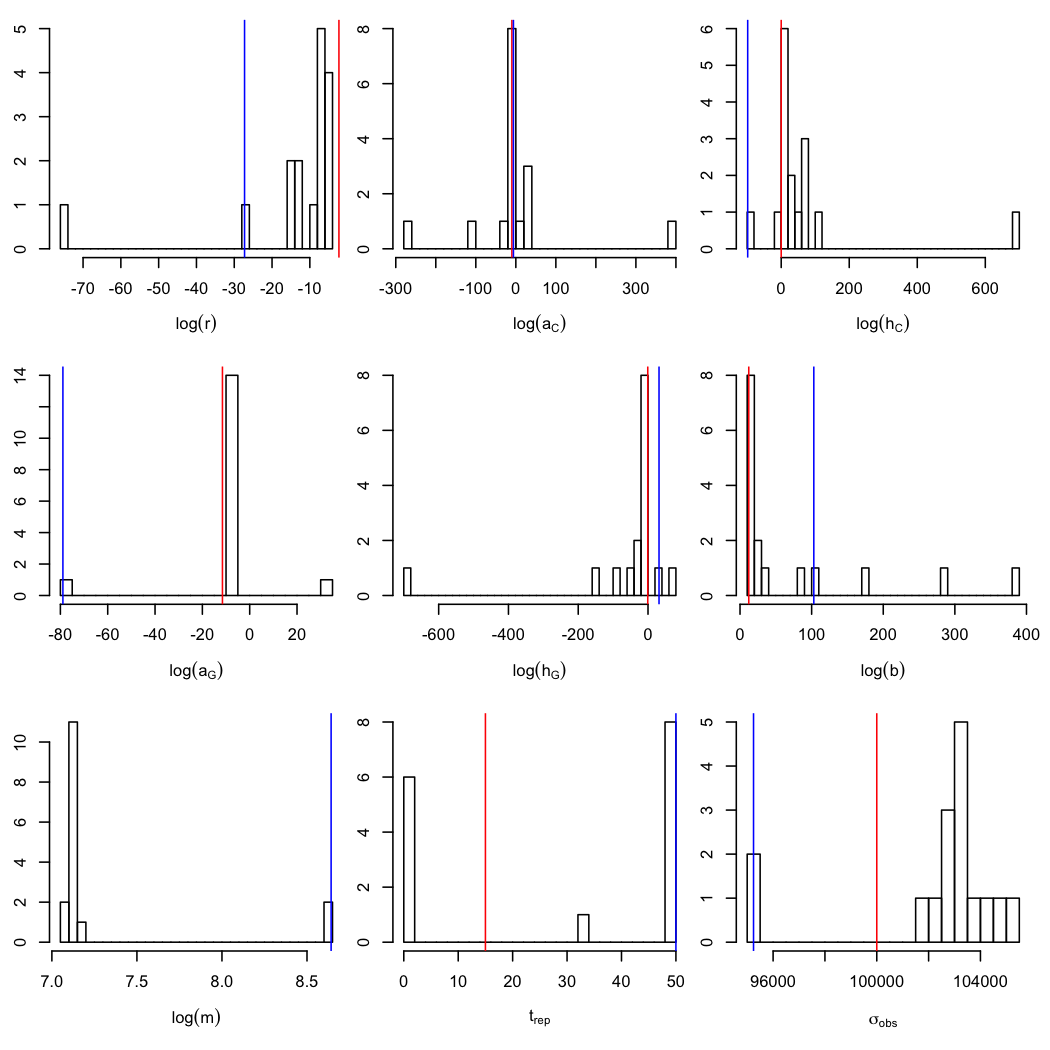
\includegraphics[width=\linewidth]{figure/hist2-1} \hfill{}

\caption[Histograms of parameter estimates for all parameter sets with log-likelihood within 5 units of the best likelihood]{Histograms of parameter estimates for all parameter sets with log-likelihood within 5 units of the best likelihood. The red line shows the true parameter value and the blue shows the parameter value for the set with highest likelihood.}\label{fig:hist2}
\end{figure}


\end{knitrout}

The other issue was whether a simpler model would actually be able to fit the data better than the more complex, data-generating model.



They key is to ask whether the structured model provides a better fit to the data than does the unstructured model.
To see that we need to compare the likelihoods of the best-fitting datasets.
However, we want to weight the likelihood differences by the number of parameters: all else equal, a model with more parameters will always be able to fit the data better.
AIC is a handy metric for such a comparison, defined as $2*k - 2\ln L$, where $k$ is the number of parameters and $L$ is the maximum likelihood.
The model with the \emph{minimum} AIC is the preferred one.
Another interesting thing to do is to ask what the likelihood of the \emph{true} parameter values is.


\begin{knitrout}\scriptsize
\definecolor{shadecolor}{rgb}{0.969, 0.969, 0.969}\color{fgcolor}\begin{kframe}
\begin{alltt}
\hlstd{AICstructured}
\hlstd{AICunstructured}
\hlstd{AICtruth}
\end{alltt}
\end{kframe}
\end{knitrout}

Here you can see that the true parameter values do provide a better fit to the observed data than do either the unstructured or the structured model.
Importantly, however, the structured model outperforms the unstructured model.
This at least gives me some confidence that data only on transmission stages might still provide enough information to support a structured over an unstructured model.



I further checked this by running 40 different parameter sets and looking at the comparison between the best-fit parameter estimates and the truth (Fig. \ref{fig:forty}).
Again, you can see that the parameters are estimated very poorly (very small, $< 10^{-5}$, and very large $>10^{10}$ parameter estimates were dropped).
However, of all of the parameters, the observation error is actually pretty well estimated.

\begin{knitrout}\scriptsize
\definecolor{shadecolor}{rgb}{0.969, 0.969, 0.969}\color{fgcolor}\begin{figure}

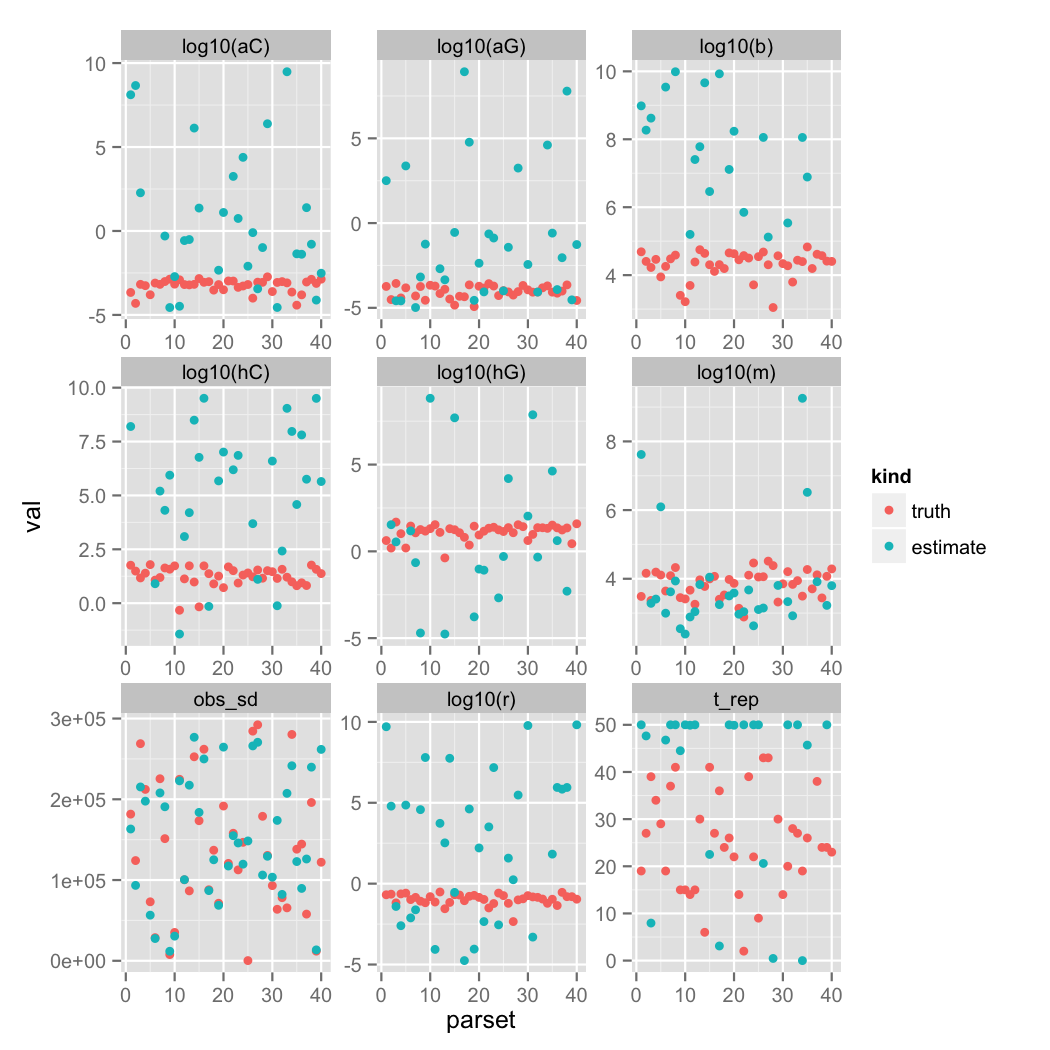
\includegraphics[width=\linewidth]{figure/forty-1} \hfill{}

\caption[Comparison of best-fit estimates to true parameter values across 40 parameter sets]{Comparison of best-fit estimates to true parameter values across 40 parameter sets.}\label{fig:forty}
\end{figure}


\end{knitrout}

Looking at the AIC across these parameter sets (Fig. \ref{fig:aiccomp}), a couple of things jump out.
First is the very small amount of variation in the structured model fits - these are typically very close to one another, suggesting that the fitting has a hard time distinguishing among parameter sets.
The structured models show much wider variation, indicative of the fact that different parameter sets produce very different dynamics.
Second is the fact that, for many parameter sets, the unstructured model has a better fit. In fact, in 35/40 cases, the unstructured model fits better than the structured model.
That suggests that, indeed, it may be hard to estimate the parameters of a structured model.
\begin{knitrout}\scriptsize
\definecolor{shadecolor}{rgb}{0.969, 0.969, 0.969}\color{fgcolor}\begin{figure}

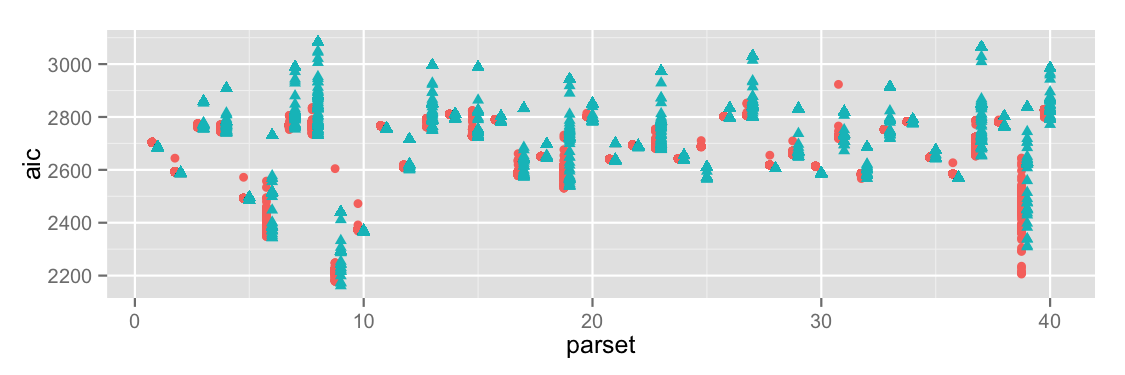
\includegraphics[width=\linewidth]{figure/aiccomp-1} \hfill{}

\caption[Comparison of structured (red) and unstructured (teal) model AIC across 40 parameter sets]{Comparison of structured (red) and unstructured (teal) model AIC across 40 parameter sets. Lower AIC is better here.}\label{fig:aiccomp}
\end{figure}


\end{knitrout}

\textbf{One thing I am concerned about is the fact that most of the structured model parameter sets had similar likelihoods}.
By assuming that every individual has identical parameters, all of the variation among individuals at sacrifice in spore load that has to be explained by observation error.
There is a considerable amount of variation in spore load at death in the real dataset, which means a lot of observation error.
I fear that this large observation error greatly expands the number of parameter sets that become plausible - with huge measurement error, even observations that are very far from the truth may be fairly likely.
This high observation error also may explain why many parameter sets have identical likelihoods even though they are different.

For a lark, I ran two parameter sets with much lower observation error, to see if this helped tighten up any of the other parameter estimates (Fig. \ref{fig:low-obs-sd-1}-\ref{fig:low-obs-sd-2}).
The short answer is, absolutely not.
For the first parameter set (Fig. \ref{fig:low-obs-sd-1}), all 1000 fit parameter sets were within 5 log-likelihood units of one another, but the parameter spread was huge.
For the second parameter set (Fig. (Fig. \ref{fig:low-obs-sd-1}), there were only 11 fit parameter sets within 5 log-likelihood units of the best, but the parameter spread was still very large.
\begin{knitrout}\scriptsize
\definecolor{shadecolor}{rgb}{0.969, 0.969, 0.969}\color{fgcolor}\begin{figure}

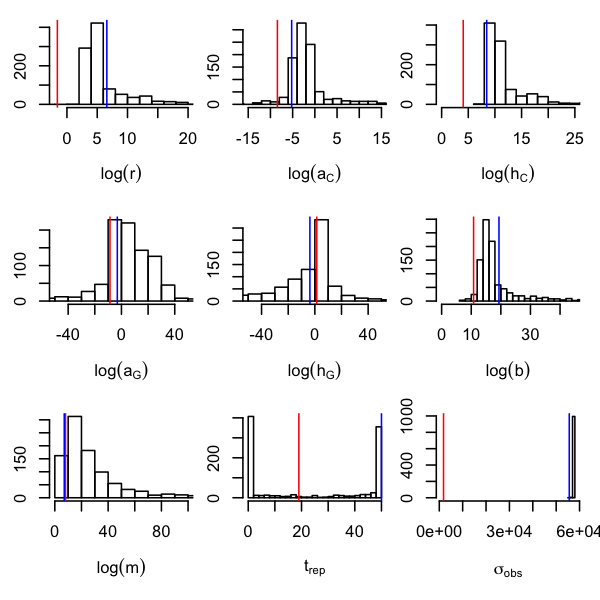
\includegraphics[width=\linewidth]{figure/low-obs-sd-1-1} \hfill{}

\caption[Parameter estimate variation when observation error is small (parameter set 1)]{Parameter estimate variation when observation error is small (parameter set 1)}\label{fig:low-obs-sd-1}
\end{figure}


\end{knitrout}

\begin{knitrout}\scriptsize
\definecolor{shadecolor}{rgb}{0.969, 0.969, 0.969}\color{fgcolor}\begin{figure}

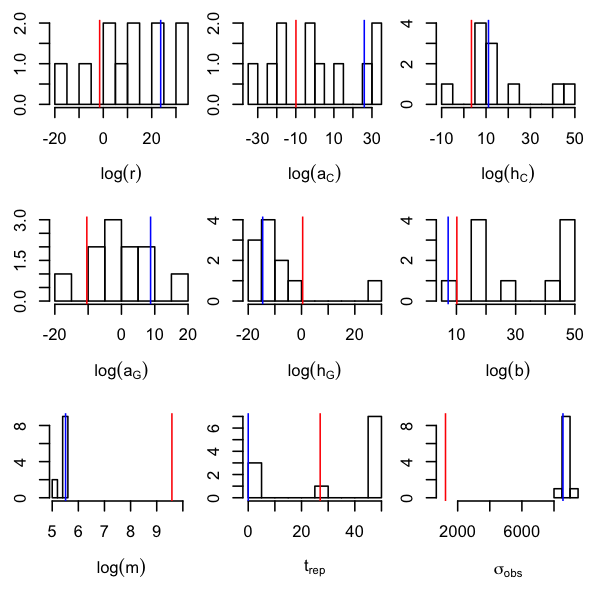
\includegraphics[width=\linewidth]{figure/low-obs-sd-2-1} \hfill{}

\caption[Parameter estimate variation when observation error is small (parameter set 2)]{Parameter estimate variation when observation error is small (parameter set 2)}\label{fig:low-obs-sd-2}
\end{figure}


\end{knitrout}

There are legitimate questions about what it may or may not be
possible to estimate using this dataset, and thus how general of a
model it will be possible to produce.
In particular, it will be impossible to estimate how long it takes for
castration to happen after exposure in this dataset because exposure
happened so early in life that none of the infected animals reproduced
at all.
I think that there will be some serious difficulties with estimating
some of the parameters without variation in the environment.
For example, I can get an equal number of transmission spores by tweaking
parameters associated with probability of infection, cauliflower stage
replication rate, and grape seed stage development rate.
If there were multiple food treatments, I could potentially
disentangle probability of infection (which should be independent of
food level) from replication/development parameters.
I'm not sure whether there will be a signal strong enough to
disentangle replication rate from development rate without information
about abundance of non-transmission stage spores.

One question is whether we seek here to develop a model that works
well for just this set of data, or whether we see k to develop a model that will work well for any dataset.
We must take advantage of the fact that ingestion is measured, so the feeding model will not be general.
A better example is that, in this dataset, castration happens prior to the onset of sexual maturity so we could, for example, assume that castration happens upon infection, ignoring the actual delay that occurs between spore ingestion and castration.
There is also the reality that, in many cases, the exposure period is long enough to consider exposure happening over a period of multiple days, such that a spore might be ingestion and not attach the first time, but then reingested later.
This would create asynchrony in developmental stages.
Again, in Cat's data, we don't really have to worry as much about that because the exposure period was relatively short compared to some of the exposure periods I have used in my experiments.
I think, for now, I will attempt to develop a model that works well
with Cat's data, and then decide how such a model needs to be extended
for more general use.

Let's think more carefully about the structure of the parasite
replication model.
In reality, what I want to consider is almost a stage-structured
model.
I feel fairly confident that each cauliflower stage corresponds to an
ingested spore that successfully penetrated the oesophagus and entered
the hemolymph.
We can therefore


\section*{DEB model}

Let's begin by laying out the standard dynamic energy budget model, and then discuss ways to include parasitism into that model.
The model begins with the dynamics of ``reserves'', a pool of metabolizable energy that is in temporary storage.
The dynamics of reserves are simple to state, and complicated to derive: the dynamics are just the difference between assimilation rate $p_A$ and mobilization rate $p_C$ (the 'C' is for 'catabolization').
\begin{equation}
\frac{dE}{dt} = p_A - p_C.
\end{equation}
The dynamics of assimilation depend on the feeding model.
For the surface-area-dependent Type II functional response common to DEB models,
\begin{equation}
p_A = \rho I_{max} \frac{F}{f_h + F} L^2.
\end{equation}
Here $\rho$ is the fraction of ingested food which is assimilated, $I_{max}$ is the surface-area-specific ingestion rate, $F$ is the density of food, $f_h$ is the half-saturation constant, and $L^2$ is surface area related to observed length.
We can safely assume that the scaling of surface area from length is incorporated into the $I_{max}$ term.
\textbf{However,} it is important to note that we are not, currently, assuming a Type II functional response.
Based on what I have seen, we are assuming a Type I functional response with a clearance rate that depends on both size and spore load.

Cat has calculated the clearance rate as $\log(F_0/F_1)*V/T$, where $F_0$ is the initial number of algae cells, $F_1$ is the final number of algae cells, $V$ is the volume of the tube, and $T$ is the duration of the feeding trial (3 hours).
This model is assuming an exponential decrease in the number of algae cells, with the rate of decrease determined by the ingestion rate of the daphnid; essentially, the daphnid has a linear functional response.
Cat also calculates a size-corrected clearance rate as the observed clearance rate divided by the square of the length, that is, assuming that clearance rate is dependent on the surface area.
\textbf{It will probably be desirable to fit a feeding model to all of this data to estimate its parameters, and also to compare alternative feeding models, although I believe that Spencer has done this to some extent already.}
In the work I have seen, Spencer fits some models that allow feeding rate to depend on spore load/infection status.
Spencer's results suggest that feeding rate should depend on the number of spores.
One thing to consider: if all the parasite's replication happens early, then the change in feeding rate through infection time has more to do with the \emph{size} of the parasite spores than their numbers (see discussion above).
\emph{A key for this study is the ability to treat the feeding model parameters as fixed, rather than needing to estimate them}; even if feeding rate changes as the abundance of spores changes dynamically.

\subsection*{A slightly-modified version of the standard DEB model}
There are lots of ways to write down the standard DEB model.
I have a version that I have used that simplifies the standard DEB model in some ways that I think are useful.
This version assumes that energy reserves $E(t$ increase due to ingestion, and are mobilized $p_C(E,V,t)$ to fuel growth in volume $V(t)$ and egg production $R(t)$.
The simplification I make to the standard DEB model is in assuming that there are no ``maturity maintenance'' costs; this prevents the possibility of a sexually mature animal ``reverting'' to sexual immaturity.
It also is beneficial for working with \emph{Daphnia}, since, to a good approximation, sexual maturity can be measured by length (that is, it is possible to define a ``size at maturity'' that applies to all individuals).

\begin{align}
\frac{dE}{dt} &= \rho I_{max} \frac{F}{f_h+F} V^{2/3} - p_C, \\
\frac{dV}{dt} &= \frac{\kappa~p_C - k_M~E_G~V}{E_G}, \\
\frac{dR}{dt} &= \frac{(1-\kappa)~p_C}{E_R}, \\
p_C &= E \left(\frac{\frac{v}{V^{2/3}} + k_m}{1+\frac{\kappa E}{E_G V}}\right).
\end{align}

This is the description of the growth dynamic under ``good'' food conditions.
In the experiments, although not technically in chemostats, I believe that food was held as close to constant as possible (daily food transfers, saturating food).
Clearance rates were also directly measured, as were size and spore load.
Because of this, we can safely remove most of the terms relating to feeding from the model.
In particular, I think we can begin by using the raw measurement of size-dependent clearance rate in place of $I_{max}~F/(f_h+F)$.
Then we can focus only on estimating the assimilation efficiency $\rho$.
We can simplify further by using the assimilation efficiency estimated for $\emph{D. pulex}$, e.g. in the the work by McCauley, Nisbet et al., as the parameter $\rho$.

\subsection*{Including parasitism}
Here is where things get a bit dicier, because we are faced with many possible ways of adding parasitism, as noted above.
To constrain ourselves a bit, let's assume that the parasite shuts off reproduction by causing all energy allocated to reproduction to instead be allocated to growth, and let's assume that the parasite, in way way or another, uses this energy as a resource.
The three issues we need to deal with are the following:
\begin{enumerate}
\item \emph{When} does the parasite shut of energy allocation to reprodution?
\item \emph{How} is the parasite population structured?
\item \emph{Where} does the parasite get its energy from growth?
\end{enumerate}

The \emph{when} question is a bit easier.
Castration is not instantaneous, as many individuals are able to have clutches (including clutches that are larger than normal) after exposure to the parasite.
However, if infection occurs early enough in life (that is, early enough before sexual maturity is reached), then castration happens prior to sexual maturity.
In the data for Cat's experiments, castration precedes sexual maturity for all individuals, so we could make the assumption that castration is instantaneous upon infection.
Or we could follow the model structure above and assume that castration happens $n$ days post-infection, letting $n$ be estimated on the basis of the data.
That is the structure I will assume now.

The \emph{how} question is also not too bad.
If the parasite population is unstructured, then we are explicitly treating the parasite population as homogeneous (which we know it is not), so all spores are transmission spores, and all spores use the same amount of energy.
I think we cannot, in good faith, use this model.
I think we must assume some simple structure (like that suggested above).
In this case, we can consider three parasite subpopulations: ``cauliflower stages'' that produce pre-transmission stages, which requires some amount of energy from the host; ``pre-transmission stage'' that develop into transmission stages, which requires some amount of energy from the host; ``transmission stages'' that are inert, simply taking up space inside the host.
To be fully general, this suggests a delay-differential equation approach, because individual infecting spores infect the host at different times and each ``cauliflower stage'' produce pre-transmission spores time; this means that pre-transmission stages (and, subsequently, transmission stages) have a distribution of ages within the host.

However, a simpler alternative is a continuous-time stage-structured population model.
We just want to make the rates of transitioning between stages (i.e., the probabilities of transitions) dependent on ingestion rates, food densities, etc.
A simple model to begin is the following:
\begin{align}
\frac{dN_C}{dt} &= p_I \times \text(clearance rate) \times N_{T,env} - \mu N_C, \\
\frac{dN_P}{dt} &= b(E,V) N_C - p_T(E,V) N_P, \\
\frac{dN_T}{dt} &= p_T(E,V) N_P.
\end{align}

In this model, the total number of cauliflower stages $N_C$ depends upon clearance rates (feeding, not immune!), the probability of infection, and the density of transmission-stage spores in the environment.
Cauliflower stage spores ``deactivate'' at a rate $\mu$.
Note that although this enters the model as a death rate, it isn't biologically a death rate - it is just a way of ensuring that cauliflower stages don't produce pre-transmission spores indefinitely.
In experiments, new cauliflower stages would only be coming in while the host was in the exposure phase.
Cauliflower stages produce pre-transmission stages $N_P$ at a rate $b$ that depends (potentially) on energy reserves and host size.
These pre-transmission stage spores transition to becoming transmission stages $N_T$ at a rate $p_T$ that may depend on reserves and host size.
Transmission stage spores persist within the host forever.
This seems like a pretty good model to begin with - it is quite simple (structurally) but roughly captures what we know about the biology of the host.
What remains is to specify functional forms for $b(E,V)$ and $p_T(E,V)$, so that they depend upon the energy being allocated to growth.

\emph{Where} exactly that energy is coming from is trickier, as I noted above.
I am working from the assumption that the energy used by the parasite comes from growth (in some capacity), rather than reserves are reproduction.
The total energy allocated to growth is $\kappa~E_G~p_C$ in DEB model (or just $p_C$ once castration happens).
Maintenance costs are subtracted from this total, and the remainder is used for growth, with a conversion cost of $E_G$.
The growth model (without parasitism) is just:
\begin{equation}
\frac{dV}{dt} = \frac{\kappa~p_C - k_m~E_G~V}{E_G}.
\end{equation}

There are several ways to incorporate parasite energy theft into growth.
Seemingly, the simplest is to assume that the parasite steals some fraction of the energy allocated to growth.
Focusing on the point after all energy is allocated towards growth (i.e., $\kappa=1$), we assume that the parasite steals some fraction $\sigma(N,E,V)$ of mobilized energy $p_C$. The remainder goes to fuel host growth. Then the model for growth and parasite population size (ignoring structure for simplicity) is something like:
\begin{align}
\frac{dV}{dt} &= \frac{(\kappa-\sigma(N,E,V))~p_C - k_m~E_G~V}{E_G}, \\
\frac{dN}{dt} &= \sigma(N,E,V)~p_C.
\end{align}
The fraction of energy stolen by the parasite could potentially depend on the number of parasites, the size of the host, the size of the host's energy reserves, or none of these things.
My results suggest that it might just be a constant fraction, regardless of the host's size or energetic state, and that the total number of parasites would depend on the host and environmental factors that affect the mobilization flux $p_C$.
However, this model becomes much more problematic when you assume that the parasite population is structured, with multiple stages using energy.
The challenge is that $\sigma(N,E,V)$ becomes $\sigma(N_C, N_P, E, V)$, where it is the sum of the two parasite populations that affect how much total energy is stolen.
Given that this is a fraction, it must remain bounded between 0 and 1.
So, for example, if you have
\begin{equation}
\sigma = \frac{a_1 N_C + a_2 N_P}{1 + a_1 N_C + a_2 N_P},
\end{equation}
that ensures that the total fraction of energy stolen cannot be greater than xsxs


The next simplest model is to assume that the parasite actually utilizes ``structure'' in some way, shape, or form, as a resource.
In this case, we let $\sigma(N,V)$ be the parasite's rate of ``structure conversion to parasite biomass'' or some other such thing, and the model for host and parasite growth becomes
\begin{align}
\frac{dV}{dt} &= \frac{\kappa~p_C - k_m~E_G~V }{E_G} - \sigma(N,V), \\
\frac{dN}{dt} &= \sigma(N,V).
\end{align}

More complicated are models where the parasite is utilizing energy that is allocated to growth in a dynamic way.
The reason this is slightly more complicated is that $\kappa~p_C$ is an energy flux; it has units of energy per time.
If we imagine the the parasite is acting as a ``predator'' on host energy, we would write down its ``functional response.''
For example, in Hall et al. 2009, Spencer had the parasite using energy reserves $E$ as a resource, and wrote down the parasite's per-capita growth rate as
\begin{equation}
a_N \frac{E}{h_N+E}-m_N.
\end{equation}
It is less obvious how to do that when the equivalent of $E$ in Hall et al. 2009 is $p_C$.
The simplest way is to simply treat $p_C$ as they did $E$.
That's fine (mathematically), but it is worth pointing out that the terms of this ``functional response'' don't have the same biological interpretation (and cannot be derived on the basis of a physical argument).
However, we will go with it for now, and say that $\sigma(N,p_C)$ is the functional response of the parasite.
There are two ways that the parasite might access energy.
\begin{align}
\frac{dV}{dt} &= \frac{\kappa~(p_C - \sigma(N,p_C)) - k_m~E_G~V}{E_G}, \\
\frac{dN}{dt} &= \sigma(N,p_C).
\end{align}
In this model, the parasite reduces the amount of mobilized energy available for growth.
The second model is
\begin{align}
\frac{dV}{dt} &= \frac{\kappa~p_C - k_m~E_G~V - \sigma(N,\kappa~p_C)}{E_G}, \\
\frac{dN}{dt} &= \sigma(N,p_C).
\end{align}
In this model, the parasite only has access to the energy that has been allocated to growth.
Of course, practically speaking, these two models will be identical because $\kappa=1$ once castration occurs.
So we can profitably reduce the number of models down to three by assuming that most (essentially, all) of the replication happens after castration has occurred.

I am also going to make an assumption that is not obvious here, which is that the mobilization rate rules do not change upon infection.
That is, the functional form of $p_C$ in infected hosts will be identical to that of uninfected hosts.
This is problematic is because the (admittedly obscure) derivation of the form of the mobilization rate equation relies on assumptions that are not met in infected hosts.
In particular, the DEB assumption of ``weak homeostasis'' is almost certainly violated.
This assumption states that, under constant food, there is a ``reserve density'' (defined by the quantity $E/V$) which remains constant.
Given that the parasite is developing inside the host, causing a rechanneling of energy and siphoning off some of that energy for itself, it seems very unlikely to imagine that the ratio of reserves to structure will remain constant.
However, previous work using DEB models to study infection (Hall et al. 2007, 2009 and Flye-Sainte-Marie et al. 2009) have not worried about this assumption violation, and those have been co-authored by DEB pioneers like Nisbet and Kooijman.
Thus, I will assume that this is not too big of a problem.

Of course, there are mathematical details that have not been made explicit yet.
In particular, we need to specify functional forms for the parasite's energy use or growth.
It seems reasonable to assume that the parasite's growth will be modeled using the Monod equation (i.e., the parasite will have a Type II functional response), since it is a microbe in an aqueous environment (the hemolymph) uptaking a limiting nutrient (energy).

Let's take each model in turn.
For simplicity, I will assume that ingestion is determined by clearance rate $a$ (which has units of volume/time) times the density of food in the environment $F$ (so $F$ has units of cells/volume).
I will also assume that this rate does not depend on size, but does depend on infection status (but not spore load).

Prior to exposure, the standard DEB model applies.
During the 24-hr exposure period, spores are ingested, but are not replicating, and the host behaves as normal.
There is some probability of infection given ingestion ($\rho_I$), and the total number of spores ingested depends on clearance rate $a$ and the density of spores in the environment $N_{env}$.
\begin{align}
p_C &= E \left(\frac{\frac{v}{V^{2/3}} + k_m}{1+\frac{\kappa E}{E_G V}}\right). \\
\frac{dE}{dt} &= a~F - p_C, \\
\frac{dV}{dt} &= \frac{\kappa~p_C - k_m~E_G~V}{E_G}, \\
\frac{dN_C}{dt} &=\rho_I~a~N_{env} - \mu N_C.
\end{align}
After exposure ends, the dynamics are again given by the standard DEB model.
This lasts for $n$ days (where $n$ is like the incubation period for the parasite).
$n$ will be estimated on the basis of the data.
After $n$ days, the host is castrated and the parasite begins replicating.
Here is where this model starts to break down, becoming much more difficult to analyze.
\begin{align}
p_C &= E \left(\frac{\frac{v}{V^{2/3}} + k_m}{1+\frac{\kappa E}{E_G V}}\right). \\
\frac{dE}{dt} &= a~F - p_C, \\
\frac{dV}{dt} &= \frac{\kappa~p_C - k_m~E_G~V}{E_G}, \\
\frac{dN_C}{dt} &= -\mu N_C
\frac{dN_P}{dt} &=
\end{align}


After some period of time $n$, the



\section*{Suggested future experiments}
Infection experiment with varying initiation of reduced food.
If I am correct that most (all) of the replication happens early in infection, then the total (transmission vs. pre-transmission) number of spores should be relatively unaffected by reductions in food late in infection.
However, the total number of transmission stages would be affected, because reducing the food late in infection reduces the developmental rate of the pre-transmission stages.
It also might increase density-dependent competition for resources.

\section*{Notes to self}
\subsection*{Derivation of the clearance model}
The clearance rate was calculated as $\log(F_0/F_T) (V/T)$, where $F_T$ is the final number of cells, $F_0$ is the initial number of cells, $V$ is the volume of the container, and $T$ is the amount of time the feeding trial lasted.
This comes from the following model of feeding (where $F(t)$ is the amount of food at any time $t$:
\begin{equation}
\frac{dF}{dt} = -a/V F(t)
\end{equation}
Implicit in this equation are the units of the parameters: $a$ is the clearance rate and has units of L/time; $V$ has units of L, and $F(t)$ has units of algal cells.
Solving and manipulating this equation:
\begin{align*}
&\frac{1}{F(t)} dF = -a/V dt \\
&\log(F(t)) = -at/V + C \\
&F(t) = F_0~e^{-at/V} \\
&F(T) = F_0~e^{-aT/V} \\
&e^{aT/V} = \frac{F_0}{F_T} \\
&\frac{aT}{V} = \log\left(\frac{F_0}{F_T}\right) \\
& a = \log\left(\frac{F_0}{F_T}\right) \left(\frac{V}{T}\right)
\end{align*}

\end{document}
